\vspace{0.5em}
\subsubsection{Mechanical Integration}
\hfill
\\
\indent The mechanical design and integration of the sensing suite were crucial to ensure stable operation, accurate data alignment, and reproducibility across experiments. 
This subsection is divided into three parts:
\begin{itemize}
    \item 3D printed mounts for flexible radar positioning.  
    \item 3D dedicated IMU mounting plate.  
    \item Geometric placement of radars and corresponding coordinate transformations.  
\end{itemize}

\vspace{0.5em}
\paragraph{Radar Mounting Design}
\hfill
\\
% -- Explain the custom 3D-printed designs that allowed adjustable yaw/pitch positioning of the radars.
% -- Show figures of the mounts and describe their role in fine-tuning sensor orientation.
% -- Emphasize stability and repeatability.
\indent A standard mounting bracket is provided by the manufacturer for the IWR6843AOP sensor, as shown in Figure~\ref{fig:IWR6843AOP_mount}. 
While suitable for simple setups, this bracket only allows a fixed mounting position without the possibility of adjusting yaw or pitch. 
Such limitations restrict the ability to optimize the radar field of view for different vehicle placements and test scenarios.  

To overcome this, a custom 3D-printed bracket was developed, enabling adjustable tilt and offering greater flexibility in sensor alignment (Figures~\ref{fig:IWR6843AOP_mounts_comparison} and \ref{fig:IWR6843AOP_3D_mounts}). 
This design provides precise control over the radar orientation, which is essential for minimizing ground reflections, extending horizontal coverage, and ensuring that both radars could be consistently aligned with the vehicle’s coordinate frame.  

The bracket consists of three main components:  
\begin{itemize}
    \item A stable \textbf{mounting base} securely attached to the vehicle platform.  
    \item A \textbf{sensor frame} that holds the IWR6843AOP in position.  
    \item An adjustable \textbf{tightening screw} that locks the tilt angle once aligned.  
\end{itemize}

The mounts were fabricated using PLA, chosen for its ease of printing and adequate stiffness for field use. 
They were fixed to the vehicle platform with hot glue, a lightweight yet sufficiently rigid method to ensure stability during operation. 
This approach minimized vibration-induced artifacts and guaranteed repeatable positioning across experiments.  

By introducing this adjustable design, the system achieved both mechanical robustness and alignment flexibility, enabling more accurate calibration of the dual-radar setup and improving consistency in downstream data fusion.  

\begin{figure}[!htbp]
    \centering
    \begin{subfigure}[t]{0.48\linewidth}
        \centering
        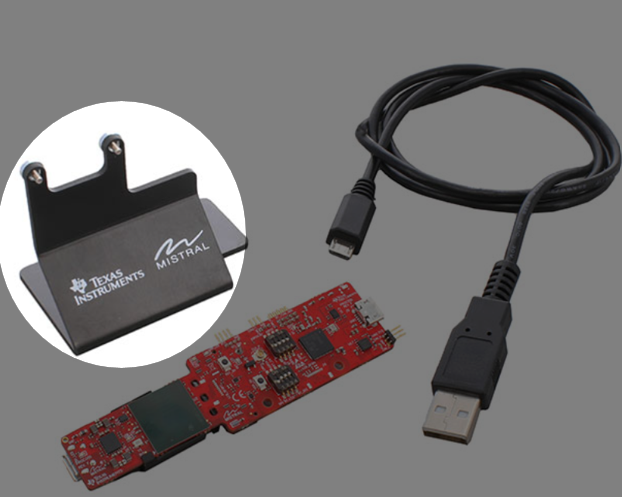
\includegraphics[width=\linewidth]{images/IWR6843Mount.png}
        \caption{Manufacturer-provided mount for the IWR6843AOP sensor. This design fixes the sensor in place without tilt adjustment, limiting flexibility.\\
        \textit{Source: amicus engineering, available at \href{https://amicus.com.sg/products/iwr6843aop-evaluation-module-for-single-chip-60ghz-antenna-on-package-aop-mmwave-sensor/}{amicus.com.sg}}}
        \label{fig:IWR6843AOP_mount}
    \end{subfigure}
    \hfill
    \begin{subfigure}[t]{0.48\linewidth}
        \centering
        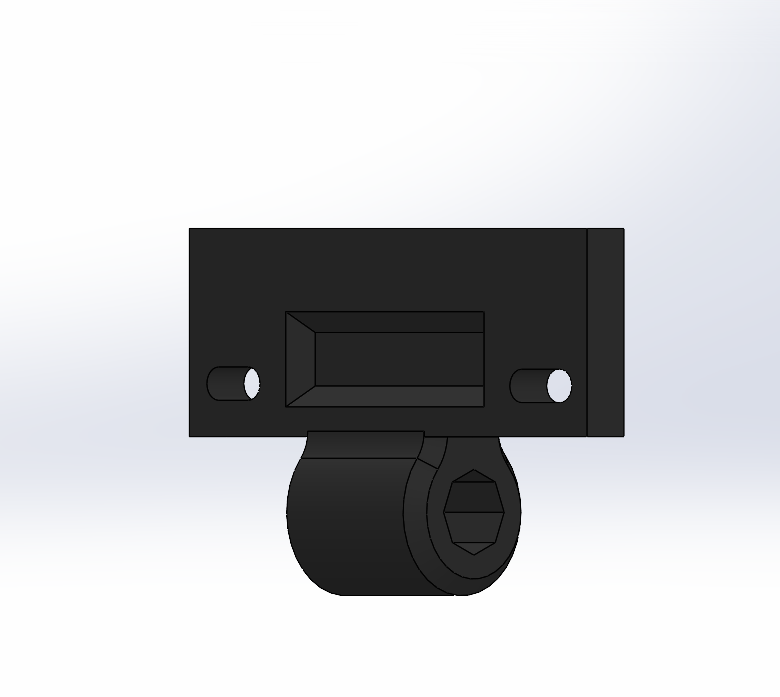
\includegraphics[width=\linewidth]{images/3DModelSensorMount.png}
        \caption{Custom 3D-printed mount designed. It enables controlled tilt adjustments, ensuring repeatable alignment and optimized field of view.}
        \label{fig:IWR6843AOP_3D_sensorMount}
    \end{subfigure}
    \caption{Comparison of sensor mounting options for the IWR6843AOP radar: (a) fixed manufacturer mount and (b) adjustable 3D-printed design. The custom bracket provides alignment flexibility and stability, improving calibration for dual-radar operation.}
    \label{fig:IWR6843AOP_mounts_comparison}
\end{figure}

\begin{figure}[!htbp]
    \centering
    \begin{subfigure}[t]{0.48\linewidth}
        \centering
        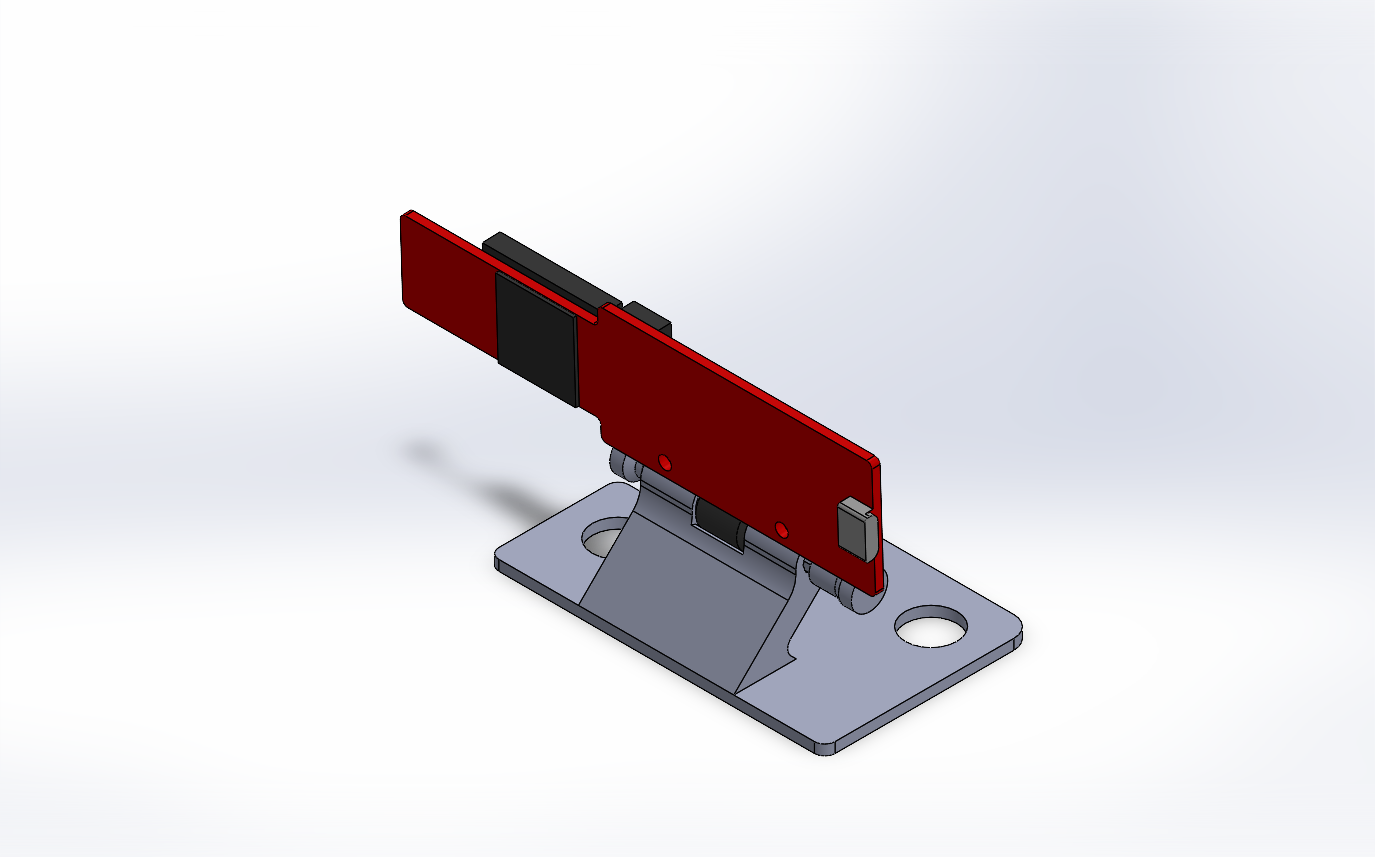
\includegraphics[width=\linewidth]{images/3DModelFullSensor.png}
        \caption{IWR6843AOP sensor mounted on the custom 3D-printed bracket in its default upright orientation. 
        The mount provides a stable base while allowing tilt adjustments.}
        \label{fig:IWR6843AOP_3D_mount}
    \end{subfigure}
    \hfill
    \begin{subfigure}[t]{0.48\linewidth}
        \centering
        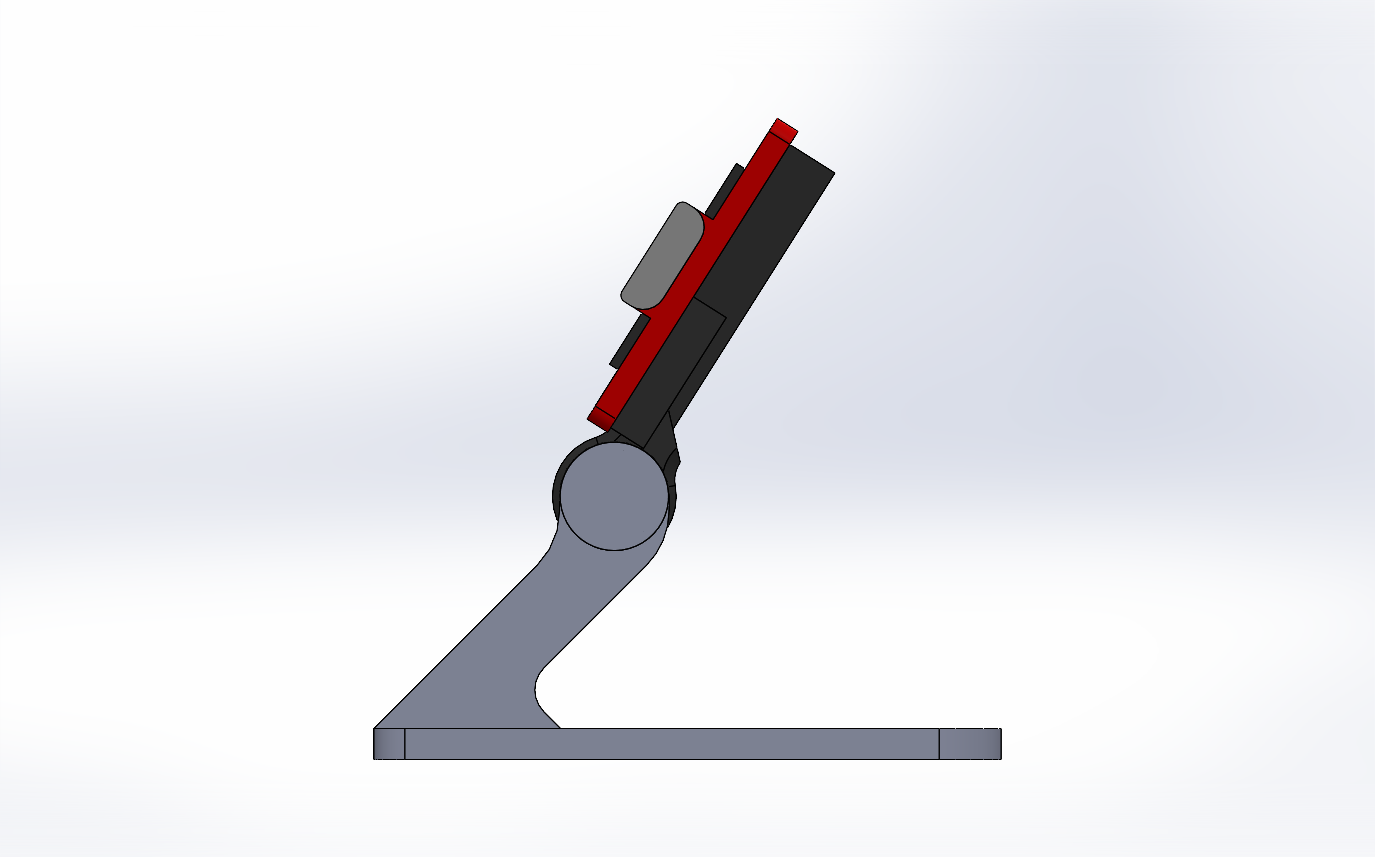
\includegraphics[width=\linewidth]{images/3DModelFullSensorSideTilt.png}
        \caption{Side view showing the tilt functionality of the custom bracket. 
        This adjustability was critical for compensating the $15^\circ$ upward tilt used in the dual-radar configuration.}
        \label{fig:IWR6843AOP_3D_mount_tilt}
    \end{subfigure}
    \caption{Implementation of the custom 3D-printed mounting solution for the IWR6843AOP radar. 
    The design combines stability with controlled tilt adjustment, enabling repeatable calibration and improved alignment with the vehicle frame.}
    \label{fig:IWR6843AOP_3D_mounts}
\end{figure}

\begin{figure}[!htbp]
    \centering
    \includegraphics[width=0.65\linewidth]{images/SensorInVehicle.png}
    \caption{Prototype installation of the IWR6843AOP radar sensor on the vehicle. 
    This early mounting solution was used for visualization and comparison with the 3D design, but it was not adopted as the final configuration.}
    \label{fig:SensorInVehicle}
\end{figure}

While the 3D model (Figures~\ref{fig:IWR6843AOP_mounts_comparison}-\ref{fig:IWR6843AOP_3D_mounts}) illustrates the intended mounting geometry, Figure~\ref{fig:SensorInVehicle} shows an intermediate real-world implementation.
This prototype installation provided a practical check of sensor tilt and positioning but was later replaced by the custom 3D-printed bracket, which ensured stability, repeatability, and precise control over yaw and pitch adjustments.

\vspace{0.5em}
\paragraph{IMU Mounting Design}
\hfill
\\
\indent The MTi-G710 IMU required a stable and horizontally aligned installation point to ensure that its quaternion orientation output could be directly mapped to the vehicle reference frame without introducing additional correction.  
To achieve this, a custom mounting solution was developed, illustrated in Figure~\ref{fig:MTi3DModel}.  

The 3D design, shown in Figure~\ref{fig:MTi3DModel}, highlights the three main elements of the assembly:  
\begin{enumerate}
    \item The MTi-G710 sensor.  
    \item A flat mounting plate designed to secure the device.  
    \item The rear vehicle mounting spot, located near the spoiler.  
\end{enumerate}

This location was selected because it provided a rigid and vibration-resistant base, while also being naturally aligned with the horizontal plane of the vehicle.  
The design ensured that the IMU could be mounted flush, minimizing installation errors and avoiding unnecessary post-processing of orientation data.  

The real-world implementation is shown in Figure~\ref{fig:MTiRealMount}, where the IMU was securely fixed to the vehicle.  
This placement offered both ease of integration and the stable reference needed for reliable sensor fusion with the radar system.  

\begin{figure}[!htbp]
    \centering
    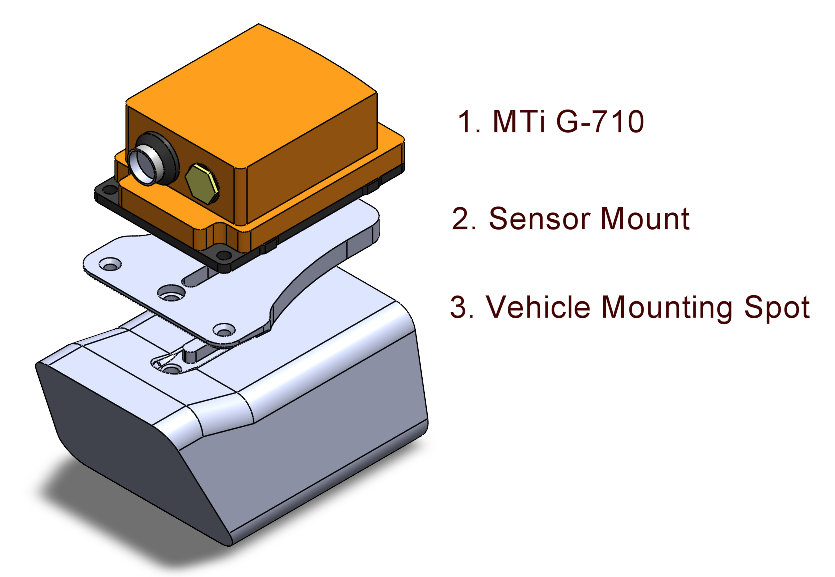
\includegraphics[width=0.65\linewidth]{images/MTi3DModel.png}
    \caption{3D model of the MTi-G710 IMU installation. 
    The design consists of (1) the IMU, (2) a custom flat sensor mount, and (3) the rear vehicle mounting spot selected for its stability and horizontal alignment.}
    \label{fig:MTi3DModel}
\end{figure}

\begin{figure}[!htbp]
    \centering
    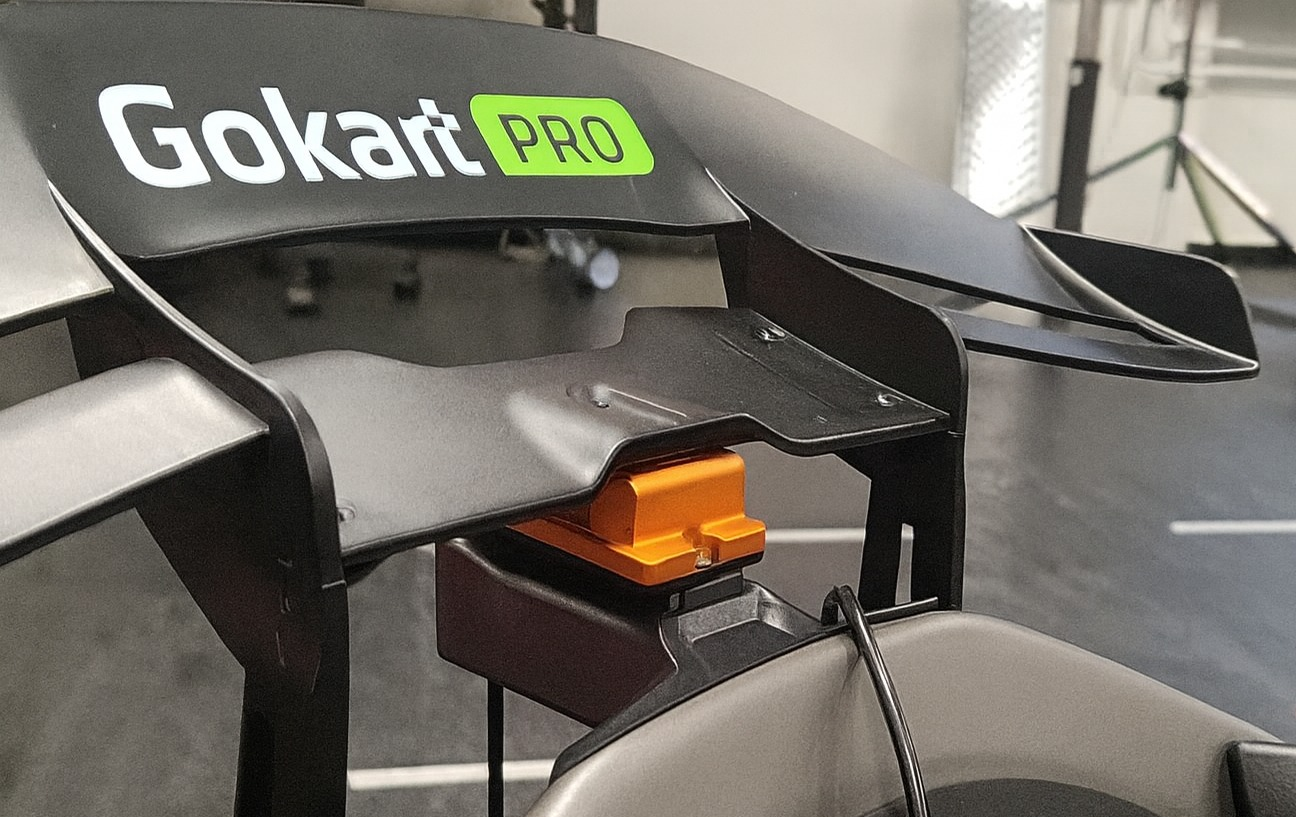
\includegraphics[width=0.65\linewidth]{images/MTiVehicleMount.png}
    \caption{Real-world installation of the MTi-G710 at the rear vehicle mount point. 
    This position near the spoiler ensured a rigid and level platform, reducing post-processing requirements for orientation correction.}
    \label{fig:MTiRealMount}
\end{figure}
